\documentclass[border=10pt]{standalone}

% --- packages (mirror these in figure.meta.json "requires") ---
\usepackage{tikz}
\usetikzlibrary{positioning, arrows.meta}

% --- palette (canonical source: reference/color-palettes/color-palettes.md; light variant) ---
\definecolor{otblue}{HTML}{0072B2}
\definecolor{otorange}{HTML}{E69F00}
\definecolor{otteal}{HTML}{009E73}
\definecolor{otpurple}{HTML}{CC79A7}
\definecolor{otgray}{HTML}{5A5A5A}

% ===== reusable icon sub-pictures (adapted from icons/) ==================
% Each is a small self-contained tikzpicture, dropped into a node so it can be
% positioned and connected by its anchors. Swap/extend with other icons.
\newcommand{\datasetpic}{%
  
\begin{tikzpicture}[line width=0.6pt]
    \fill[otteal!8] (0,0) rectangle (1.3,0.9);
    \filldraw[draw=otteal!75!black, fill=otteal!22] (0,0.9) rectangle (1.3,1.2);
    \draw[otteal!55] (0.433,0)--(0.433,1.2) (0.866,0)--(0.866,1.2)
                     (0,0.3)--(1.3,0.3) (0,0.6)--(1.3,0.6);
    \draw[draw=otteal!75!black, line width=0.8pt] (0,0.9)--(1.3,0.9) (0,0) rectangle (1.3,1.2);
  \end{tikzpicture}}
\newcommand{\gpupic}{%
  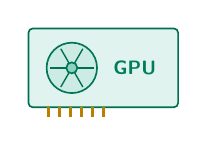
\begin{tikzpicture}[line width=0.6pt]
    \filldraw[draw=otteal!70!black, fill=otteal!12, rounded corners=1.5pt] (0,0) rectangle (1.9,1.0);
    \begin{scope}[shift={(0.55,0.5)}]
      \filldraw[draw=otteal!75!black, fill=otteal!20] (0,0) circle[radius=0.32];
      \foreach \a in {0,60,...,300}{\draw[otteal!70!black, line width=0.5pt] (0,0)--(\a:0.28);}
      \filldraw[draw=otteal!75!black, fill=otteal!45] (0,0) circle[radius=0.07];
    \end{scope}
    \node[font=\sffamily\scriptsize\bfseries, text=otteal!80!black] at (1.35,0.5){GPU};
    \foreach \i in {0,...,5}{\draw[otorange!80!black, line width=1pt] (0.25+\i*0.14,0)--+(0,-0.12);}
  \end{tikzpicture}}
\newcommand{\serverpic}{%
  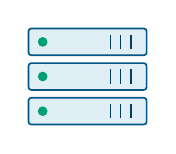
\begin{tikzpicture}[line width=0.6pt]
    \foreach \i in {0,1,2}{
      \filldraw[draw=otblue!75!black, fill=otblue!12, rounded corners=1pt]
        (0,\i*0.44) rectangle (1.5,\i*0.44+0.34);
      \filldraw[otteal] (0.18,\i*0.44+0.17) circle[radius=0.05];
      \foreach \j in {0,1,2}{\draw[otblue!55!black, line width=0.5pt]
        (1.5-0.2-\j*0.13,\i*0.44+0.08)--+(0,0.18);}
    }
  \end{tikzpicture}}
% ========================================================================

\begin{document}
% ==== parameters (edit these) ============================================
\def\colsep{4.6}    % horizontal gap between stages: data -> workers -> server (cm)
\def\rowsep{2.5}    % vertical gap between GPU workers (cm)
% labels
\def\datalabel{Training data}
\def\workeronelabel{Worker 1}
\def\workertwolabel{Worker 2}
\def\workerthreelabel{Worker 3}
\def\pslabel{Parameter server}
\def\batchlabel{batch}
\def\gradlabel{$\nabla\theta$}
\def\weightlabel{$\theta$}
\def\titlelabel{Distributed data-parallel training}
% =========================================================================

\begin{tikzpicture}[
    >={Stealth[length=2.4mm]},
    icon/.style={inner sep=1pt},
    slbl/.style={font=\sffamily\footnotesize, text=otgray},
    data/.style={draw=otgray!75, line width=1pt, ->},
    grad/.style={draw=otpurple!85!black, line width=1pt, ->},
    wts/.style={draw=otteal!70!black, line width=1pt, ->, dashed},
  ]

  % data source
  \node[icon] (data) at (0,0) {\datasetpic};
  \node[slbl, below=2pt of data] {\datalabel};

  % GPU workers
  \node[icon] (w1) at (\colsep, \rowsep)  {\gpupic};
  \node[icon] (w2) at (\colsep, 0)        {\gpupic};
  \node[icon] (w3) at (\colsep, -\rowsep) {\gpupic};
  \node[slbl, below=2pt of w1] {\workeronelabel};
  \node[slbl, below=2pt of w2] {\workertwolabel};
  \node[slbl, below=2pt of w3] {\workerthreelabel};

  % parameter server
  \node[icon] (ps) at (2*\colsep,0) {\serverpic};
  \node[slbl, below=2pt of ps] {\pslabel};

  % data sharding: dataset -> workers
  \draw[data] (data.east) -- (w1.west);
  \draw[data] (data.east) -- (w2.west) node[midway, above, slbl] {\batchlabel};
  \draw[data] (data.east) -- (w3.west);

  % synchronisation: gradients up to the server, weights back down (curved apart)
  \foreach \w in {w1,w2,w3}{
    \draw[grad] (\w.east) to[bend left=10] (ps.west);
    \draw[wts]  (ps.west) to[bend left=10] (\w.east);
  }
  \node[slbl, text=otpurple!85!black] at (1.5*\colsep,0.6)  {\gradlabel};
  \node[slbl, text=otteal!70!black]   at (1.5*\colsep,-0.6) {\weightlabel};

  % title
  \node[font=\sffamily\bfseries] at (\colsep,{\rowsep+1.2}) {\titlelabel};

\end{tikzpicture}
\end{document}
